% !TEX TS-program = pdflatex
% !TEX encoding = UTF-8 Unicode

% This is a simple template for a LaTeX document using the "article" class.
% See "book", "report", "letter" for other types of document.

\documentclass{sig-alternate}
%\usepackage[margin={1.5cm,3cm}]{geometry}
%\setlength{\columnsep}{1cm}
\usepackage[utf8]{inputenc} % set input encoding (not needed with XeLaTeX)

%%% Examples of Article customizations
% These packages are optional, depending whether you want the features they provide.
% See the LaTeX Companion or other references for full information.

%%% PAGE DIMENSIONS
%\usepackage{geometry} % to change the page dimensions
%\geometry{a4paper} % or letterpaper (US) or a5paper or....
% \geometry{margin=2in} % for example, change the margins to 2 inches all round
% \geometry{landscape} % set up the page for landscape
%   read geometry.pdf for detailed page layout information
%\usepackage[hidelinks]{hyperref}
%\usepackage[autostyle,french=guillemets,babel]{csquotes}
\usepackage{graphicx} % support the \includegraphics command and options
\usepackage[backend=biber]{biblatex}
\addbibresource{biblio.bib}
% \usepackage[parfill]{parskip} % Activate to begin paragraphs with an empty line rather than an indent
%%% PACKAGES
\usepackage{booktabs} % for much better looking tables
\usepackage{array} %
% for better arrays (eg matrices) in maths
\usepackage{paralist} % very flexible & customisable lists (eg. enumerate/itemize, etc.)
\usepackage{verbatim} % adds environment for commenting out blocks of text & for better verbatim
%\usepackage{subfig} % make it possible to include more than one captioned figure/table in a single float
% These packages are all incorporated in the memoir class to one degree or another...
\usepackage{amsfonts}

%%% HEADERS & FOOTERS
\usepackage{fancyhdr} % This should be set AFTER setting up the page geometry
\pagestyle{fancy} % options: empty , plain , fancy
\renewcommand{\headrulewidth}{0pt} % customise the layout...
\lhead{}\chead{}\rhead{}
\lfoot{}\cfoot{\thepage}\rfoot{}

%%% SECTION TITLE APPEARANCE
%\usepackage{sectsty}
%\allsectionsfont{\sffamily\mdseries\upshape} % (See the fntguide.pdf for font help)
%% (This matches ConTeXt defaults)

%%% ToC (table of contents) APPEARANCE
%\usepackage[nottoc,notlof,notlot]{tocbibind} % Put the bibliography in the ToC
%\usepackage[titles,subfigure]{tocloft} % Alter the style of the Table of Contents
%\renewcommand{\cftsecfont}{\rmfamily\mdseries\upshape}
%\renewcommand{\cftsecpagefont}{\rmfamily\mdseries\upshape} % No bold!

%%% END Article customizations

%%% The "real" document content comes below...

\title{ Bridging [TBD]}

\author{
% You can go ahead and credit any number of authors here,
% e.g. one 'row of three' or two rows (consisting of one row of three
% and a second row of one, two or three).
%
% The command \alignauthor (no curly braces needed) should
% precede each author name, affiliation/snail-mail address and
% e-mail address. Additionally, tag each line of
% affiliation/address with \affaddr, and tag the
% e-mail address with \email.
%
% 1st. author
\numberofauthors{3}
\alignauthor
Alex Palesandro\\
\affaddr{Orange Labs, France}\\
\texttt{alex.palesandro@gmail.com}
\alignauthor
Aurélien Wailly\\
\affaddr{Orange Labs, France}\\
\texttt{aurelien.wailly@orange.com}
\alignauthor
Marc Lacoste\\
\affaddr{Orange Labs, France}
\texttt{marc.lacoste@orange.com}
}
%\setlist[itemize]{leftmargin=*}
\begin{document}
\maketitle

\abstract{
%Today, hypervisors have to find a complex trade-off between functionalities provided and security assurance. Those requirements are contrasting by design:
%adding new features will generally increases the LoC and consequently the attack surface. On the contrary, those code additions are required to properly fulfill market requests. 
%
%Nested virtualization is a technique capable to diversify hypervisor features. Exploiting an extra layer of virtualization, we will be able to decouple different requirements, avoiding the need to find delicate trade-off.
%
%In this paper, we will analyze the state of nested virtualization in modern hypervisor and evaulating the impact of utilization of microhypervisor to enforce a stronger security level.
The problem of homogeneity over multiple IaaS providers is receiving considerable attention with the evolution toward nested virtualization. These new architectures unveil user-centric opportunities such as efficient resources management and VM migration. However the inherent drawbacks hinder its global adoption with a larger TCB and the complexity to monitor another virtualization layer. Thus, we argue that the promising architectural view of micro hypervisors approach is the key to the separation of hypervisor duties and reducing the attack surface.

Furthermore, our architecture mushrooms commodity and micro hypervisors to leverage nested virtualization in terms of user-data privacy, modularity, TCB size and compatibility. These design principles are evaluated for each architecture configuration and compared to establish a reference security architecture. The resulting combination is built over common hypervisors empowered with micro hypervisors features. A reference implementation proven the architecture to be viable and will be extended to meet broader hypervisor scopes, enabling migration over heterogeneous cloud servers.
}

\section{Introduction}
\label{ref:intro}
Cloud computing platform are a solid reality nowadays. Modern cloud platforms are able to provide elastic use of resources, optimizing their allocation in order to meet the user needings. However, currently deployed cloud platforms present still several limitation. 

First, it is still difficult to deliver cloud applications which are able to transparently leverage over several platform resources. The concept of SuperCloud~\cite{art:blan, xclo:blank} addresses this kind of problems. Multi-platform coordination primarily for different standard and several format lock-in. Unfortunately, those lock-in are not only due to market strategical decisions but they also reflects the virtualization technology heterogeneity. For example, each cloud provider could use a different storage system or a different format to store VMs images. Different hypervisors have nowadays a low degree of compatibility between them and this generally prevents leveraging on some popular features like `` VM live migration'' between different platform. Moreover, this incompatibility could also be enlarged if we consider that several platforms adopts one or more different virtualization techniques. In addition, this situation induce a tight dependency between the customer and the cloud provider and hardens the possibility to guarantee the availability of service in presence of a certain provider or to put in place some geographical optimization due to cost or traffic origin. The result was that some data server failures in the past has been catastrophic, causing a prolonged outage of service for a plenty of applications.. In the remaining part of the work, we will refer to those issues as ``horizontal'' requirements, that shows straightforwardly their multi-platform nature.

The second class of issues concerns platform integrity and user data privacy. On one hand, from an user-centric point of view, the user would like to preserve privacy of its data when it stores data on the cloud platform. However, hypervisor is normally the most privileged task executed in the platform and therefore a curious or malicious administrator could easily retrieve those data~\cite{cloudvisor:zhang}. Moreover, in multi-tenancy cloud platform, a user shares the same physical resources with other users. Several works~\cite{sec:you, bot:att} showed the potential threat and risks of attacks issued by other users located on the same physical resource.
On the other hand, from a user-centric point of view, it is difficult to observe and inspect deeply the functioning of the whole platform, leveraging commodity general purpose hypervisors (GPHs).GPHs are executed at the most privileged level and so, it is complicated to detect and intervene on them in presence of malicious attack or misbehavior, without service interruption for all VMs hosted on the server. 
To sum up, both visions collide with the execution of the hypervisor at the highest level of privileged. This attitude prevents the platform administrator from a real monitoring of the whole platform, but also the possibility for users to concretely inspects actions that platform administrators do on user data. A major challenge of new generation cloud platform is to alleviate this different tension, finding an acceptable trade-off. In the following paragraphs, we will make reference to this class of problem as ``Vertical'' requirements.

To resume, in order to present a complete view of the architecture, we identified five key design principles, that a cloud computing platform has to implement in order to solve the cited problems. In the following paragraphs, those principles will represent a grid of analysis of different architectures.
\begin{itemize}[]
\item \textbf{DP1 User-Data privacy} A curious or malicious administrator ( or another platform user) would not have the right to inspect and analyze user data and instances, without the explicit consensus with the user above mutually trusted services. User-data privacy is a major challenge of modern cloud platforms. It is important to identify a trade-off that allows providers to identify and intervene on possible menaces, but also guarantee the impossibility for a curious or malicious operator to access to them without restrictions. In order to respect this principle when a platform administrator manages the platform it has not the highest level of privilege and each action on users object that he wants to deliver has to be validated by a mutually-trusted core, executed at the highest level of privilege. Moreover, this mutually-trust core has also to apply memory page cipher/uncipher in order to prevent memory page snooping when a page is swapped out.
\item \textbf{DP2 Fail-Safe modular architecture} In order to recover soft failures, the archtecure is supposed to be fail-safe, being able of automatically migrate instances or user-data in presence of a menace, but also reactivating the correct functioning in presence of a software failure. In order to satisfy this property, the amount of safety-critical components has to be as lowest as possible and the overall design has to be kept as modular as possible
\item \textbf{DP3 Small TCB} The amount of lines of code executed at the highest level of privilege is normally proportional to the number of potential failures and bugs in the platform. According to this, an architecture presenting a tiny TCB will improve its safety and integrity properties by design.
\item \textbf{DP4 Inter-platform support} The cloud architecture has to be designed in order to support directly different platforms and service providers. The same user virtual instances have to be executed (and potentially migrated) unmodified over different platforms.
\item \textbf{DP5 3rd part compatibility} Avoid disruption of existing 3rd part applications compatibility could represent a major principle to consider. Platform interfaces has to be kept as close as possible to the existing one, preventing application rewrite.
\end{itemize}
Moreover, beside this functional design principles specifying which features have to be achieved by the platform, another set of non-design principles could be identified. Those principles does not concern directly features or aspects of the architecture of the platform, but the effective feasibility of the architecture. 
\begin{itemize}[]
\item \textbf{NDP1 Minimize code addition} a major issue could be represented by the amount of code lines that have to be added and maintained to an existing architecture to meet the functional requirement. Even it does not represent strictly a technical limitation to a certain proposal, it could become a ``show-stopper'' factor for its utilization.
\end{itemize}
In our analysis, it will be kept in consideration not only the overall suitability of the architecture, but also a quantification of the effort needed to develop and deploy it. In table \ref{int:des} it is possible to observe a resume of previous cited principles.
 
\begin{table}
\label{int:des}
\begin{tabular}{llll}
\toprule
Id & Functional design Principle & Class &\\
\midrule
   DP1 & User-Data privacy & Vertical & \\
   DP2 & Fail-Safe modular architecture & Vertical & \\ 
   DP3 & Small TCB & Vertical & \\
   DP4 & Inter-platform support & Horizontal & \\
   DP5 & Backwards 3rd part compatibility & Horizontal \\
   NDP1 & Minimize code addition & & \\
\bottomrule
      \end{tabular}
\end{table}

This paper is organized as following. In Section~\ref{sec:rw} we analyze the nested virtualization ecosystem and position existing solutions regarding our design principles. In Section~\ref{classic}, we details limitations of classical nested virtualization approach and in Section~\ref{sec:mh} we present the microvisor approach. In Section~\ref{sec:archcomp} we compare cloud architectures propositions, combining nested virtualization and microvisors, leveraging the design principles grid introduced before.
%Furthermore, in Section 6 we define a security architecture for multi-cloud scenario, with an analysis of necessary software components to satisfy vertical design principles.
In Section~\ref{sec:conclu}, we conclude the paper with future works and our vision of the SuperCloud.
% in section in section 6 we define a security architecture for multi-cloud scenario, with an analysis of necessary software components to satisfy vertical design principles. In section 8, we conclude the paper with future works in section 8.
 
\section{Related Work}
\label{sec:rw}
% Intro + performance issues
Several works presented in literature integrates these a subset of this design principles in their architecture, leveraging nested virtualization \cite{turtle:ibm,art:blan, cloudvisor:zhang}
Cloud computing feature set could be enlarged exploiting two layers of virtualization instead of just one. The presence of two different hypervisors allows the possibility to specialize hypervisors functions. Instead of having a general purpose hypervisor we could split the hypervisor role in two different layers, interconnected with a well defined interface.
Each layer will have to care about a subset of features, simplifying overall development.
However, nested virtualization on x86 architecture faced impeding performance issues \cite{rec:virt}.

% Perfomance issuess adressed
However, several works demonstrate that it is possible to put in place low overhead nested virtualization using special approaches \cite{turtle:ibm} . Moreover, other works try to recover performance loss exploiting multi-level consolidation, introduced in nested virtualization \cite{art:blan}. In conclusion, nested virtualization slowdown could be considered nowadays an acceptable price to achieve advanced features and, in addition, hardware manifacturers are developing and proposing new hardware facilities to reduce this overhead \cite{vmcs:nakajima}.

To sum up, no architecture had been presented to address vertical and horizontal class of problems at the same time until now. XenBlanket does not investigate cloud architectural security concerns (DP3,DP2), limiting the focus on new potential feature of a coordinated multi-provider cloud. Cloudvisor proposed a security architecture that leverages nested virtualization without allowing the possibility of executing more than one nested hypervisor at time, that is a crucial requirements of a multi-provider cloud platform (DP4). In a SuperCloud scenario, each user has to run its own L1 hypervisor instance to enforce a compatibility layer, overcoming incompatibilities between different providers.

Other approaches leveraging only one layer of virtualization does not achieve the whole design-principle satisfaction. Self-service cloud approach (SSC) \cite{ssc:art} design a complete security architecture to overcome major security and privacy issues of currently deployed cloud infrastructures, in order to alleviate the different needing user-centric and provider-centric vision of cloud computing presented in \ref{par:intro}. Even if this architecture reproduces an approach similar to the SuperCloud without leveraging an extra layer of virtualization (DP4), the approach changes the behavior where the user acts introducing new components that have to be directly managed by the user. Therefore, the main drawback of this solution is to change the interface with the user, preventing the possibility to straightforwardly move to the new platform without having to change its applications (DP5).

% Integration NDSS Taming
Furthermore, DeHype \cite{wu2013TamHosHypMosDepExe} presented a dissected version of KVM hypervisor, trying to reduce the TCB of this popular hypervisor. The approach consisted in demoting a great part of the hypervisor codebase to a user-level execution. DeHype satisfies all vertical design principles listed before (DS1,DS2,DS3), reinterpreting the microkernel approach of demoting the greatest part of code to userspace. DeHype increases a lot the robustness of a cloud platform leveraging KVM, limiting for example the possibility of attack in multi-tenancy platform, but it does not address horizontal design principles about a multi-provider service.

\section{Classic nested virtualization approach}
\label{sec:classic}

Nested virtualization refers to a system architecture with two layers of virtualization. It consists in a ``virtualized'' virtualization, where the guest system virtualize a nested guest. The concept could be generalized to an arbitrary number of nested guest layers, introducing recursive virtualization.
%More formally, Popek \& Golberg \cite{Popek:1974:FRV:361011.361073} discussed this subject, introducing the concept of ``recursively virtualizable'' machine and giving an initial definition of recursive virtual machines: If it is possible for a virtual machine to run under itself a copy of the VMM that could also exhibit all the properties of the VMM and this procedure could be repeated until the resources of the systems are consumed, then the original machine is recursively virtualizable.

Introducing nested virtualization, we have to identify the two main actors involved in the virtualization process: bare-metal hypervisor (L0) and nested hypervisor (L1). In addition, we will refer to the nested guest as L2 guest. 
However, virtualization introduces a computational overhead. It is small when we are dealing with single layer virtualization, but it grows exponentially when we try to add further levels \cite{rec:virt}. This huge performance overhead has prevented nested virtualization adoption during last years and had been finally addressed by Ben Yehuda et Al \cite{turtles:ibm} proposing an architecture with acceptable overhead.

Nested virtualization feasibility opened a plenty of new possibilities and perspectives, that have been largely discussed in literature \cite{rec:virt,turtles:ibm,art:blan}. The first aspect in common among different works proposed in literature is to diversify hypervisor functions, introducing new features but keeping the existing ones. In a general analysis of existing works, it could be possible to identify the general role of each different layer.
On one hand, L0 is charged of the vertical aspects of the platform. It has to achieve  the best possible performances and enforcing the strongest possible level of isolation. L0 represents the last line of defense of the platform and a privileged point of global status observation.

On the other hand, L1 is responsible for horizontal feature set. it has to provide the widest possible support to different platforms and the capacity to virtualize adopting different techniques ( para-virtualization, hardware-assisted, dynamic binary translation). According to these requirements, Williams et al. \cite{art:blan} propose a patched version of Xen, Xen Blanket, to accomplish a L1 virtualization layer, designed to run over different platforms. This concretely allows to run over different physical platform the same VM, and live-migrate it at the occurrence.

\subsection{Classical nested virtualization limits}

Nowadays, nested virtualization presents several limits related to the hardware support and software state of implementation. At first, to provide nested virtualization, hypervisors has to provide an exact copy of hardware virtualization facilities. The most exploited technique, full virtualization with hardware assistance (HV), relies on a quite complex dedicated support.
This set of facilities assists instruction emulation, memory address translation and device management. Both Xen and KVM propose nested VMX/SVN features, that consists in the possibility to efficiently handle nested hardware virtualization, in presence of a single-layer hardware facilities.
%To address this performance problems, several hardware producers proposed new facilities, like Intel VMCS shadowing, that reduces the amount of nested VMEXIT when handling a nested guest VMEXIT.
Although nested virtualization performance are still not good and the feature is not yet stable on modern hypervisor \cite{xen:test}, the feature is under heavy development and it will be hopefully in a usable state soon.

Secondly, due to the monolithic architecture, each feature introduced in GPH enlarges the TCB. Therefore, leveraging GPH, a huge amount of code is running in the most privileged mode and has to be trust. Several works discuss and analyze the overall TCB of modern GPH \cite{nova, xmhf}, considering GPH TCB always bigger than 100 KLoC. This approach directly collides with one design principles introduced in the introduction paragraph (DP3), 
%that identified a small TCB as a major requirement for a solid architecture.
%A brief comparison of TCB of widespread GPH is depicted in figure \ref{fig:tcbchart}. 
%More importanly, this is particularly true looking at the monolithic approach of commercial hyper-visors, where any addition to the hypervisor body enlarges the TCB.

Finally, the above architecture does not improve the overall stability of the infrastructure. The underlying core, L0, has the same problem of single-layer GPH architecture: the large TCB implies also that a failure experienced in one of the critical components will simply produce a generalized failure of the whole platform, not satisfying DP2. Moreover, in GPH standard architecture, the administrator has the entire control of the platform and could potentially snoop and inspect user VM status and data.

This kind of architecture, in particular, does not leverage completely the possibility to hide behind a compatible layer, a really modular architecture with only a tiny critical core.
To sum up, current nested virtualization limits are represented by a certain lack of dedicated feature in modern hypervisor and the impossibility to rely on a tiny TCB (DP3,DP4).
The first one is being addressed by hypervisor developers. The second one could simply not be achieved with modern hypervisors. 

\section{Microhypervisor}
\label{sec:mh}

%\begin{figure}
%\caption{GPH TCB comparison \cite{nova}}
%\label{fig:tcbchart} 
%\begin{center}
%\includegraphics[width=\columnwidth]{figures/TCBchart.png}
%\end{center}
%\end{figure}

% Xen and KVM TCB
Consequentially, several works focused this problem leveraging a micro-hypervisor architecture, with a traditional microkernel-like design that tries to consistently reduce the amount of code running with the highest privilege level. A micro-kernel traditionally consists in a tiny core running in Kernel Mode, offering only few fundamental services to other modules running (scheduling, IPC, memory management) in a less privileged domain. All other components, in particular device drivers, are moved out in user-space.
Microkernels had been questioned because of the wasteful performance of first generations, due to IPC intrinsic cost. This argument had been completed confuted by Liedtke in 1993: \cite{liedtke1993ImpIPCbyKerDes,liedtke1995micCon}.

Microkernels have the capacity of easily redesign the hierarchy of privileges. A user application has normally to trust the tiny micro-kernel and only the set of user-space software it uses. However, this set of trusted set of drivers and tools have not to be trusted by every application executed in the system. Normally, this allows microkernels to implement different ``personalities''. User applications shares the system but could have to deal with completely different system services in a transparent way. However, ``personalities'' interest had been hugely reduced by the fact that system services, device drivers and even application had to be completely re-conceived to fit this new design pattern. Therefore, with the introduction of VMs, microkernels lost the battle in favor of hypervisors, in terms of popularity. However, the great advantage of tiny TCB, provided by microkernel, was not provided also by hypervisors. As we analyzed before, they present normally a monolithic architecture, like the great part of modern OS. This feature kept alive the interest in microkernels, in particular trying to couple microkernel benefits with virtualization.

Therefore, leveraging this concept of microkernels, a micro hypervisor (MH) is composed from a small kernel providing only essential functions, like scheduling, IPC, memory management and VMX extension. Several micro-hypervisor have been proposed in literature \cite{xmhf, nova}. They rely on the micro-kernel paradigm, extending it to virtualization. MH naturally satisfy vertical design principles (DP1,DP3, DP4). The tiny core could be considered the only system-critical componente of the architecture and, due to its relative small dimension and the consequent minor attitude to vulnerabilities,it could represent the ``last line of defense''.

In addition, MH inherits the concept of micro-kernel to implement different ``personalities''. Those ``personalities'' are concretely a set of ``processes'' handling specific functions running in user-space. As those functions are implemented outside the kernel, each user could rely on a different instances of the hypervisor user-space process, that could coexist at the same time. This process separation between user could enforce a straightforward mechanism to neutralize VM-to-VM attack from a malicious user. Moreover, user-space processes are easier to debug with commodity tools (GDB, valgrind).
Finally, this extraction process drives to a more solid platform, considering that user-space crashes are generally not fatal for the entire system integrity.  A possible example, that will be analyzed in next section, is the user-space VMM component of Nova, Vancouver, that resides in user-space \cite{nova}.
In addition, this approach is not far from the one proposed in DeHype \cite{wu2013TamHosHypMosDepExe}, where a consistent part of the KVM hypervisor has been demoted in user-space.

\subsection {MH general issues}

Despite the positives, MH approaches had demonstrated some limitations. Firstly, the straightforward one is the initial lack of hardware support, lack of device drivers are still a relevant Achilles' heel for this solutions, inherited from its ancestors microkernels. Fortunately, this kind of issue could be addressed leveraging I/O passthrough techniques, although it will cause exclusive allocation issues.

Moreover, as reported in previous sections, several cloud computing issues are simply not addressable with general purpose hypervisor (GPH). However, they are commonly widely adopted and represent the bedrock of existing platform. Therefore, GPH exports wide and solid interfaces leveraged by a plenty of different software that is able to properly communicate and act through them on the virtualization layer. On the contrary, MH lack of cloud toolkit integration, requiring an explicit support to be written, not satysfing 3rd part compatibility requirements (DP5). GPH are tightly connected with cloud toolkit and could present solid interfaces to communicate with different tools. 

Finally, microkernel modularization introduce a major challenge in architecture design. Due the increased complexity, for sake of kernel size, MH could generally lack of several virtualization features, commonly available on modern GPH hypervisor. For instance, XMHF does not support multiple guests. This kind of drawbacks could limits the potential interest in MH, even they are able to introduce several important features.

\section{Architecture comparison}
\label{sec:archcomp}

\begin{figure*}
\begin{center}
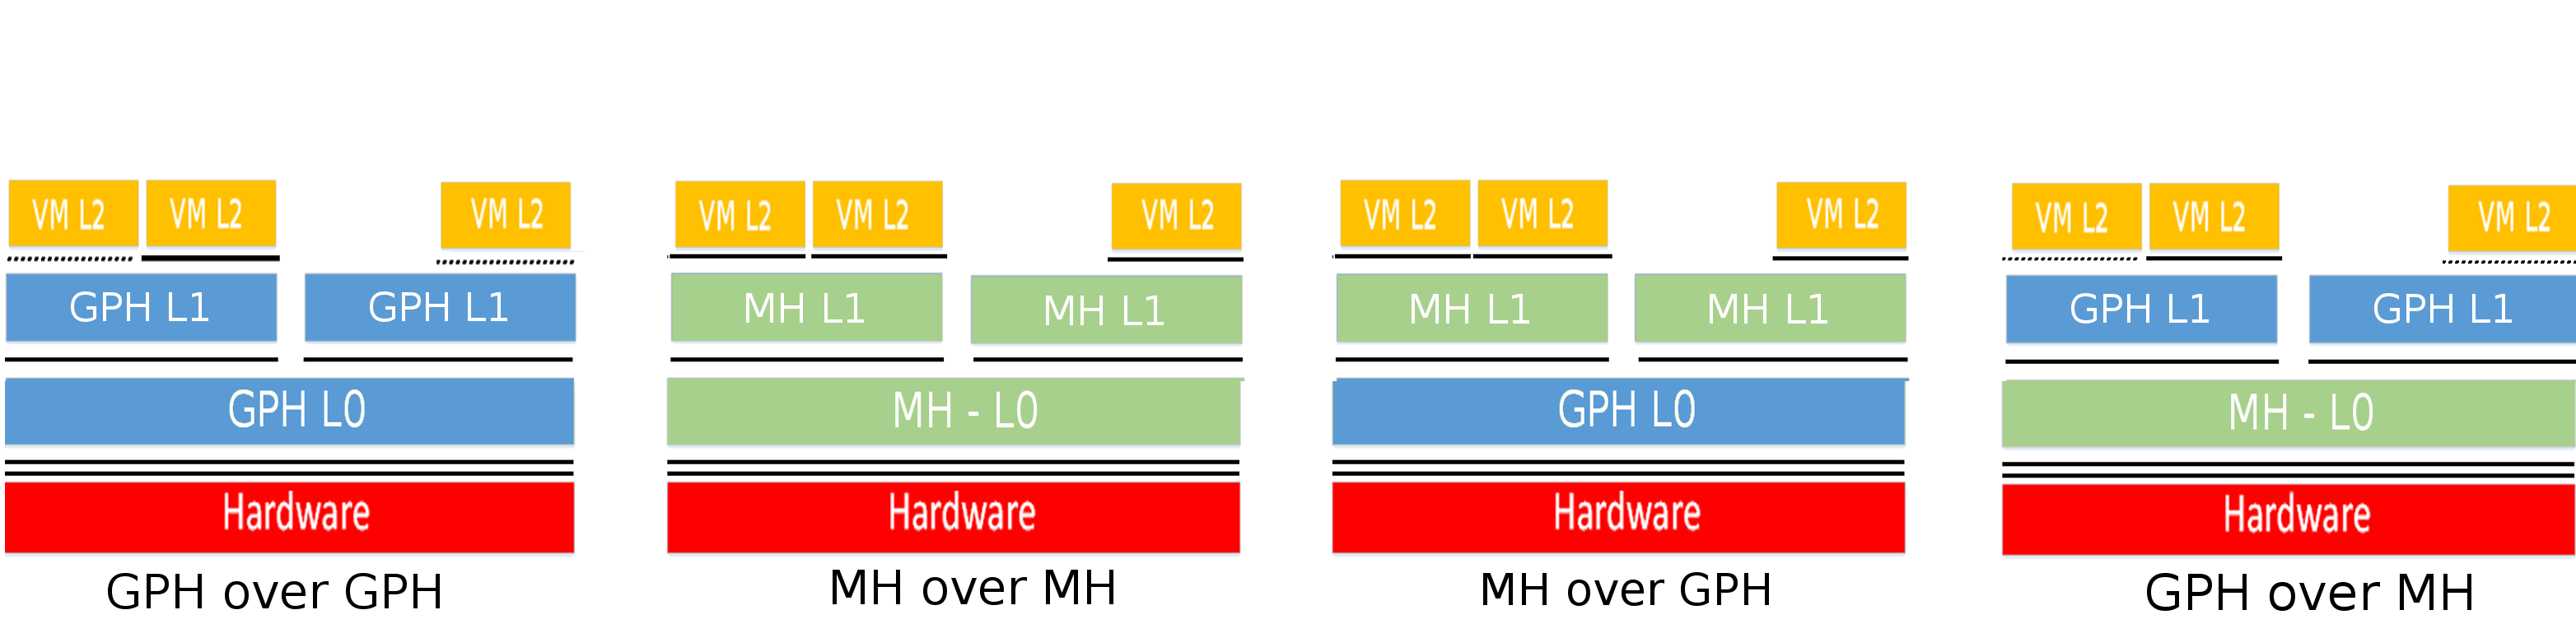
\includegraphics[width=2\columnwidth]{globalcut.png}
\end{center}
\caption{}
\label{fig:io}
\end{figure*}

The adoption of an extra layer of virtualization is capable to introduce a remarkable set of new features but it does not reduce the dimension of Trusted Code Base (TCB).
MH could represent a new approach to improve the potential benefits provided by the adoption of nested virtualization. In the following subsections, it will presented the four possible architectures achievable ``nesting'' of GPH and MH, underlying potentialities, drawbacks and potential cost of implementation.

\subsection{GPH over GPH}

The first analyzed architecture concerns only GPH. At first, it is important to recall the most interesting achievable by such architectures. In particular, several remarkable features are live migration over different platform, transparent migration of virtualized clusters between different data-centers (horizontal requirements DP1).
Supposing the completeness and the correctness of nested virtualization hardware facilities in widespread hypervisor, GPH over GPH satisfies all horizontal design principles, but it lacks in vertical DPs as the size of TCB is the same of currently deployed architectures.

To sum up, it could be possible to achieve live-migration between different platform and other features related to VM management flexibility but it could not still be possible to reduce the TCB. Analyzing MH approaches, the aim is try at most to retain to features, trying to introduce isolation and privacy improvements due to the lower TCB promised.

%Although this architectures presents an extra layer between the nested guest, normally controlled by the cloud user and the system critical part, L0, the latter is far from a satisfying security level. The TCB of KVM that is represented by the entire Linux Kernel is normally around 200 KLoCs, considering the medium size of a deployed Linux kernel.
%Moreover, default KVM configuration does not provide a transparent protection mechanism between different VMs, so that compromising one instance of QEMU, that is executed in user-space, an attacker could compromise all the others VMs on the platform.

\subsection{MH over MH}

MH on MH in reported only to see the orthogonality between this approach and GPH over GPH.
A theoretical implementation of MH over MH will provide the vertical requirements that are missing in the previous approach. The tiny core could be able to overcome monolithic problems due to privilege level of adminitration tasks (DP1), the possibility to improve the resilience of the platform to a large set of software failures (DP2) and finally reduce the possibility of the vulnerabilities of the most privilege part of the software (DP3). However, the interest on such architecture is limited because it is not able to overcome any cited issues of single-layer MH. Moreover, several horizontal properties are theoretically achievable but they will require a huge effort in developing functions of interest. Moreover, the lack of nested VMX functionalities prevents to concretely test this kind of architecture, because MH normally rely on VMX facilities in order to create a nested HVM guests.
To conclude, nested virtualization is exploited in order to fill eco-systems gaps with GPH but MH over MH does not provide any improvement in this sense.

\subsection{MH over GPH}
\label{par:mog}

The third architecture, proposed in order to reduce security concerns, is built combining an GPH at L0 and a MH at L1. 
%Several MH are proposed in literature focusing on different .
%Therefore, this model tries to exploit microhypervisor as L1 hypervisor in order to enforce better isolation between L2 and L0. L1 will exploit the emulated nested VMX provided by GPH L0 and virtualize L2. 
%With this approach, we try to isolate the attacker in a VM virtualized on a secured layer, in order to prevent attacks to L0. The attacker would have to face with an essential virtualization layer and it would not be able to attack the back-end virtualization layer. 
An interesting point of this approach is the fact of being easily be deployed, without requiring any extra code addition to the GPH, L0.  Existing GPH-based platforms could potentially exports nested VMX features to those guests. Even if this is not so usual in modern cloud platform, this lack is considered temporary and related only to the experimental status of those features.

However, the amount of code running in L0 kernel space is still as big as before and, therefore, no TCB reduction. 
Finally, adopting a MH as L1 prevents to use inter-platform enhanced features. As analyzed when dealing with MH design, the price of having a tiny core is normally paid with a lack of certain functionalities. For example, XMHF only supports one single guest. It could be easily noticed that this approach is not architecturally able to provide any new "horizontal" features, leveraging on nested virtualization. Therefore, the architecture is only able to provide the same features that are provided by today deployed ones, with an enhanced but not sufficient level of isolation.

\subsection{GPH over MH}

\label{par:gom}

\begin{table*}
\label{fin:conf}
\centering
\begin{tabular}{llcllll}
\toprule
Id & Functional design Principle & Class & GPH over GPH & MH over MH & MH over GPH & GPH over MH\\
\midrule
DP1 & User-Data privacy & Vertical & $\times$  & $\checkmark$ & $\times $ & $\checkmark$ \\
      DP2 & Fail-Safe modular architecture & Vertical & $\times$  & $\checkmark$ & $\times$ & $\checkmark$ \\
   DP3 & Small TCB & Vertical &  $\times$& $\checkmark$ & $\times$ & $\checkmark$ \\
   DP4 & Inter-platform support & Horizontal & $\checkmark$  & $\times$ & $\times$ & $\checkmark$ \\
   DP5 & 3rd part compatibility & Horizontal & $\checkmark$  & $\times$ & $\times$ & $\checkmark$ \\
   NDP1 & Minimize code addition & - & $\checkmark$  & $\times$ & $\times$ & $\checkmark$ \\
\bottomrule
      \end{tabular}
\end{table*}

In this configuration, the TCB is smaller than other architectures, due to the modular structure of micro-kernels., executed at L0. Leveraging as L1 a GPH, like Xen or KVM, provides to the user an environment apparently  identical to the one used in production today, satisfying DP5. The L1 GPH is normally integrated with modern cloud toolkits like OpenStack and will support 3rd part applications.
Therefore, the architecture presents a stronger isolation leveraging on nested virtualization, providing in particular a strong tiny core(DP3). The MH layer will be transparent from the user and it will not not any change in the functioning of the platform.

The first class of possible drawbacks of this architecture is represented by the necessity to expose to the L1 nested hypervisor the nested VMX extension to let him ``nest'' another HVM guest. This is experimentally done by GPH like Xen and KVM, but it is generally not included in the essential features provided by a minimal micro-hypervisor. As reported in XMHF paper \cite{xmhf}, the amount of lines of code for nested VMX is around 1KLOC. 
More generally, from an architectural point of view, the general MH minimalist attitude could represent a limitation to general preservation of existing platform functions. The constraint of privileged code size forces normally MH developers to drop some features, considered not essential. Therefore, several limitations could arise not only for nested virtualization proper features, but also for other class of features. For instance, XHMF is able only to virtualize one L1 instance at time. This is acceptable if the platform objective is limited to be provided of a secure core, but dramatically limits the possibility of having a platform model able to give the user the possibility to run its proper hypervisor as L1.

Another important class is the necessity to explicit hardware devices support. Device drivers represents a general Achilles' heel of MH, due the general cost of development. However, this class of problem could be addressed leveraging device assignment. L1 GPH hypervisor will handle the real device, using the proper driver now demoted to run in a lower level of privilege. It has to be underlined that this solution could represent a feasible approach only if it possible to overcome the exclusive allocation trouble (SR-IOV).
 
\subsection{Conclusion}

To conclude, this section provides a short comparison between different platforms, contrasting architecture features above the two main different types of benefits given by nested virtualization, as reported widely in literature \cite{art:blan, nested:berghmans,  cloudvisor:zhang, turtle:ibm}. The first could be identified in the augmented degree of isolation the architecture could enforce between host OS and the "customer" point of access, allowing to redesign the security architecture of the whole platform. The second one is represented by the possibility to leverage multiple virtualization layers to easily define inter-platform policy and operations between different platforms.
In table \ref{fin:conf}, it is possible a summary of the previous analysis. To conclude, GPH over MH is the most interesting one in order to enlarge nested virtualization promised benefit. This architecture with a solid and secured MH as L0 is the only able to reduce the platform TCB and this could be a key point to obtain more protected infrastructure, .
Firstly, adopting a MH as architecture trusted core, we will have a secure layer guaranteeing that administrator could not lose the control of the system. Klein et Al. \cite{Klein:2009} have demonstrated that a kernel with less than 10KLoC could be formally verified, under several conditions. This is far from be achievable today with standard GPH over GPH approach where the core is not tiny and the TCB is an order of 
magnitude bigger than MH \cite{nova}. 

However, the effort to set up a GPH over MH is strongly dependent on which technique leveraging for virtualizing L2. As stated in paragraph \ref{par:gom}, with L2 guest virtualized with the hardware assitance technique, the most popular one, the MH needs to export nVMX at least. 
On the contrary, adopting paravirtualization/Dynamic binary translation for L2 does not necessitate a particular hardware support and so it could not be necessary patch the MH to set up a platform. 
However, it has not be underestimated, however, that para-virtualization supports only a subset of OS, and could not be considered a general solution and DBT has shown important overhead.
%The last point of interest is related to device management. If MH act as L0 hypervisor, it has to deal with hardware devices, and this could necessitate of a significant code writing. In fact, there are several technologies, like Direct Assignment, allowing to bypass hypervisor control of a device. Those techniques are useful but they reduce the flexibility in the device management, requiring for example exclusive allocation of a device to a guest. To contrast this drawbacks, PCI-E propose the possibity to multiplex device with a set of virtual devices called virtual functions proposed to the L0 hypervisor, that will relax the contraint of exclusive allocation. Unfortunately this approach could not give the same flexibilty given by other techniques, like para-virtualization 
%With MH over GPH, MH could directly assigne devices to GPH that is able to implement  para-virtualize device, for example. 
%This will relief the MH of a part of devices management, giving to the GPH the responsibility to drive concretely the device but without losing interesting features. Therefore, we will need a limited amount of code to handle device without have to deal with each specific device.

To sum up,  the adoption of MH could  increase feature set introduced by nested virtualization adoption. The first impeding problem is the implementation of MH, able to propose to guest to virtualize with hardware assistance. In next section, we present an implementation of GPH over MH, that try to circumvent this limitation leveraging paravirtualization.
 \section{Implementation}
In the previous sections we proposed a functional analysis of cloud architecture in order to respect design principles that we identified in the introduction. In this section, we propose a GPH over MH implementation, based on Xen over NOVA.


\begin{itemize}[]
\item \textbf{Inter-platform support} Executed as L1, Xen would virtualize its nested guest initially using PV delivering the compatibility layer.
\item \textbf{Tiny TCB} The NOVA kernel will represent the only part of the platform executed at the highest level of privilege. Even the VMM, Vancouver, will be executed in the L0 user-space. The micro-kernel in L0 enforces a strictly modular approach to L0. Therefore, the VMM will present distinct processes instances for each L1 guest, enforcing a context division.
\item \textbf{3rd part compatibility} From a user point of view the architecture still exports the same interfaces provided by the Xen hypervisor, allowing the user to keep its applications unchanged.
\item \textbf{Fail-safe components architecture} Moreover, the tiny core is the only safety-critical software component. The system could potentially be able to recover any crash in different user-space components.
\end{itemize}

%
%%
%%%%Improving the Status Quo
%Udo Steinberg NOVA 6
%Virtualization layer is critical. Make it as small as possible.
%Design Principles:
%1)Fine-grained functional decomposition
% Microhypervisor (privileged)
% Multiple user-level VMMs (unprivileged)
% User-level drivers, applications (unprivileged)
%2)Principle of least privilege among all components
% Capability-based authorization model
%Ideas adopted from the microkernel world
%Those still existing limitations to nested HVM, made we focus on nested PV.
%Leveraging on the new architecture presented we propose a security architecture based on Xen and NOVA. 
%
%Xen is a well-known and wide-used hypervisor that is the base of several of most important cloud platforms.  We focus in particularly on the Xen support for para-virtualization. 
%
%Available from the first version of Xen in 2003, PV does not requires any specific hardware facilities. Even if some features drop in Amd64 architecture leaded to a little performance loss for PV compared to HVM guests, the real limit of PV is represented by the impossibility to virtualize Windows and other proprietary operating systems.
%However this technique is currently still exploited in widespread cloud platform like Amazon EC2.
%
%NOVA is a tiny micro-hypervisor able to virtualize several guests. It is a recent but promising open-source project developed at Technische Universitat Dresden. The aim of project is double: minimize the amount of code running in kernel mode and try boost virtualization.
%
%NOVA implements some interesting features, in particular from security point of view. It adopts a capability-based authorization model in order to implement the principle of least privilege among components. It supports SMP guests, VT-d Direct device assignement and NPT/EPT.
%
%The modular architecture of NOVA allows also to enforce a increased separation between different L1 guest. Leveraging the modular architecture of NOVA, each L1 guest communicates directly with a separate instance of the Virtual Machine Monitor, component of the hypervisor executed in user space. 
%
%The concept is to boot and use Xen as L1 hypervisor, inside a NOVA VMs. Xen hypervisor will be able to virtualize complete PV guests in a secured Cloud Platform. The presence of NOVA is completely transparent for the user.  

%Therefore, leveraging NOVA as L0 our platform could propose inter-platform features to the user. We have the opportunity to exploit a complete cloud toolkit with the Xen hypervisor implementing features like inter-platform migration and improved redundancy, as described in the Xen Blanket approach.

\section{Conclusion and future Works}
\label{sec:conclu}

%Future works will firstly concern the study of available MH, trying to identify which project could be suitable to act as L0 in a GPH over MH platform. As underlined previously, the key feature of L0 MH will be the capacity of having a tiny TCB. Moreover, additional requirements concerns the flexibility in terms VMs ( number of VM supported at the same time, CPU handling, I/O management). Finally, another criteria for choosing the L0 hypervisor will be the evaluated effort needed for integrating a nested HV extension the to the base project.
%On the other hand, L1 choice is much simpler. Previous analysis identified Xen as the most suitable hypervisor for this role. The capacity to support different virtualization techniques added to the ability of running without HV support, makes Xen suitable to act as compatibility layer. 
%
%After this initial study, the first step will be deploying a minimal nested architecture testing ``out-of-the-box'' features and limitations. The following part will concern the conception of patch and extensions in order to adapt the general design of MH to properly act as L0.
%The final goal is to provide an architecture able to leverage nested virtualization cloud platforms improvements, having a smaller TCB and allowing customers to leverage flexible migrations and scheduling.


%\section{Conclusion}
%{\scriptsize
%\bibliographystyle{abbrv}
%\bibliography{biblio}
%}
\end{document}
